\section{Environment estimators}
\label{sec:env}
% =====================================================================

Both estimators are evaluated on the \emph{full periodic box}, and on the same set of $N_r = N_g$ uniform random points (fixed seed, drawn in the unit cube and rescaled to the box, so that the random points are identical in all cosmologies up to the AP rescaling).

\subsection{ASTRA split}

The galaxies and random points are joined into a single catalogue and Delaunay-triangulated. For every point (galaxy or random), with $N_{\rm data}$ and $N_{\rm rand}$ the numbers of galaxies and randoms among its Delaunay neighbours,
\begin{equation}
r = \frac{N_{\rm data}-N_{\rm rand}}{N_{\rm data}+N_{\rm rand}} \in [-1,1].
\label{eq:astra_r}
\end{equation}
A point surrounded by galaxies ($r\to1$) lies in a dense region, a point surrounded by randoms ($r\to-1$) in an underdense one. In the original ASTRA classification \cite{ASTRA}, thresholds on $r$ define voids, sheets, filaments and knots; here we use $r$ as a continuous environment variable. The triangulation is computed independently in each subvolume (Section~\ref{sec:clustering}) on a region padded by $30\Mpch$ on each side, with periodic wrapping across the faces of the box, and $r$ is kept only for the points inside the subvolume. This removes the edge effects of a non-periodic triangulation (missing neighbours, elongated boundary simplices). The mean inter-point separation of the joint catalogue is $\simeq10\Mpch$, so the padding contains several layers of neighbours (convergence in Section~\ref{sec:robustness}).

\subsection{Density split}

As a reference we use the standard density split \cite{Paillas2023}. The galaxies are assigned to a periodic mesh of $5\Mpch$ cells with a cloud-in-cell (CIC) scheme, the overdensity field is smoothed with a Gaussian kernel of radius $R_s=10\Mpch$ by FFT, and the smoothed density contrast $\delta_R$ is read (CIC) at the position of every galaxy and random point.

\subsection{Environment quartiles}

For each method, each subvolume and each population, points are ranked by their environment value ($r$ or $\delta_R$) and split into four quartiles of exactly equal size, Q1 (most underdense) to Q4 (most overdense). Because $r$ is a ratio of small integers, many points share the same value; ties are broken at random. We consider two populations, ranked separately so that the thresholds of one do not depend on the other:
\begin{itemize}
\item \textbf{random quartiles}: the random points ranked by their environment, the query points of density split, sampling environments by volume;
\item \textbf{galaxy quartiles}: the galaxies ranked by their own environment, sampling environments by mass.
\end{itemize}

\subsection{Cosmic-web classes and why we use quartiles}
\label{sec:classes_def}

ASTRA was designed to classify points into four cosmic-web classes with fixed thresholds on $r$ \cite{ASTRA}: voids ($r\le-0.9$), sheets ($-0.9<r\le0$), filaments ($0<r\le0.9$) and knots ($r>0.9$). We use exactly the definition of the reference implementation (Eq.~\ref{eq:astra_r} with $N_r=N_g$, $r$ from a single random catalogue, these thresholds). On the DESI-like fiducial catalogue the classes are extremely unbalanced (Figure~\ref{fig:map}): 0.25\% of the random points are voids, 65\% sheets, 34\% filaments and 0.05\% knots; for the galaxies 0.07\%, 49\%, 51\% and 0.3\%. In Quijote, 0.7\%, 72\%, 27\% and 0\% of the random points. In practice the classification reduces to \emph{two dominant classes}, sheets and filaments, i.e.\ to a split of $r$ at zero; the voids and knots contain a few hundred points per subvolume, too few for precise clustering measurements (Figure~\ref{fig:classes_mp}). This imbalance motivated the use of equal-size quartiles of $r$ in the main analysis, which keep the ranking of the environments by ASTRA while giving every environment the same statistical weight, as in density split.

The ASTRA paper reports 7--11\% of random points in voids \cite{ASTRA}, against 0.25--0.7\% here. Its samples are 11--73 times denser than our LRGs (number densities $1.7\times10^{-3}$ to $1.1\times10^{-2}\,{\rm Mpc}^{-3}$, against $1.5\times10^{-4}\,{\rm Mpc}^{-3}$). The fractions are not set by the density alone (the Quijote halos, ten times sparser than the LRGs but more strongly clustered, have more voids), but by the density contrast of the tracer field at the scale of the mean inter-point separation. This is another manifestation of the adaptive scale of ASTRA (Section~\ref{sec:robustness}): fixed thresholds on $r$ do not select the same environments in samples of different density and bias, whereas quantiles of $r$ do define comparable environments.


\begin{figure*}[!tp]
\centering
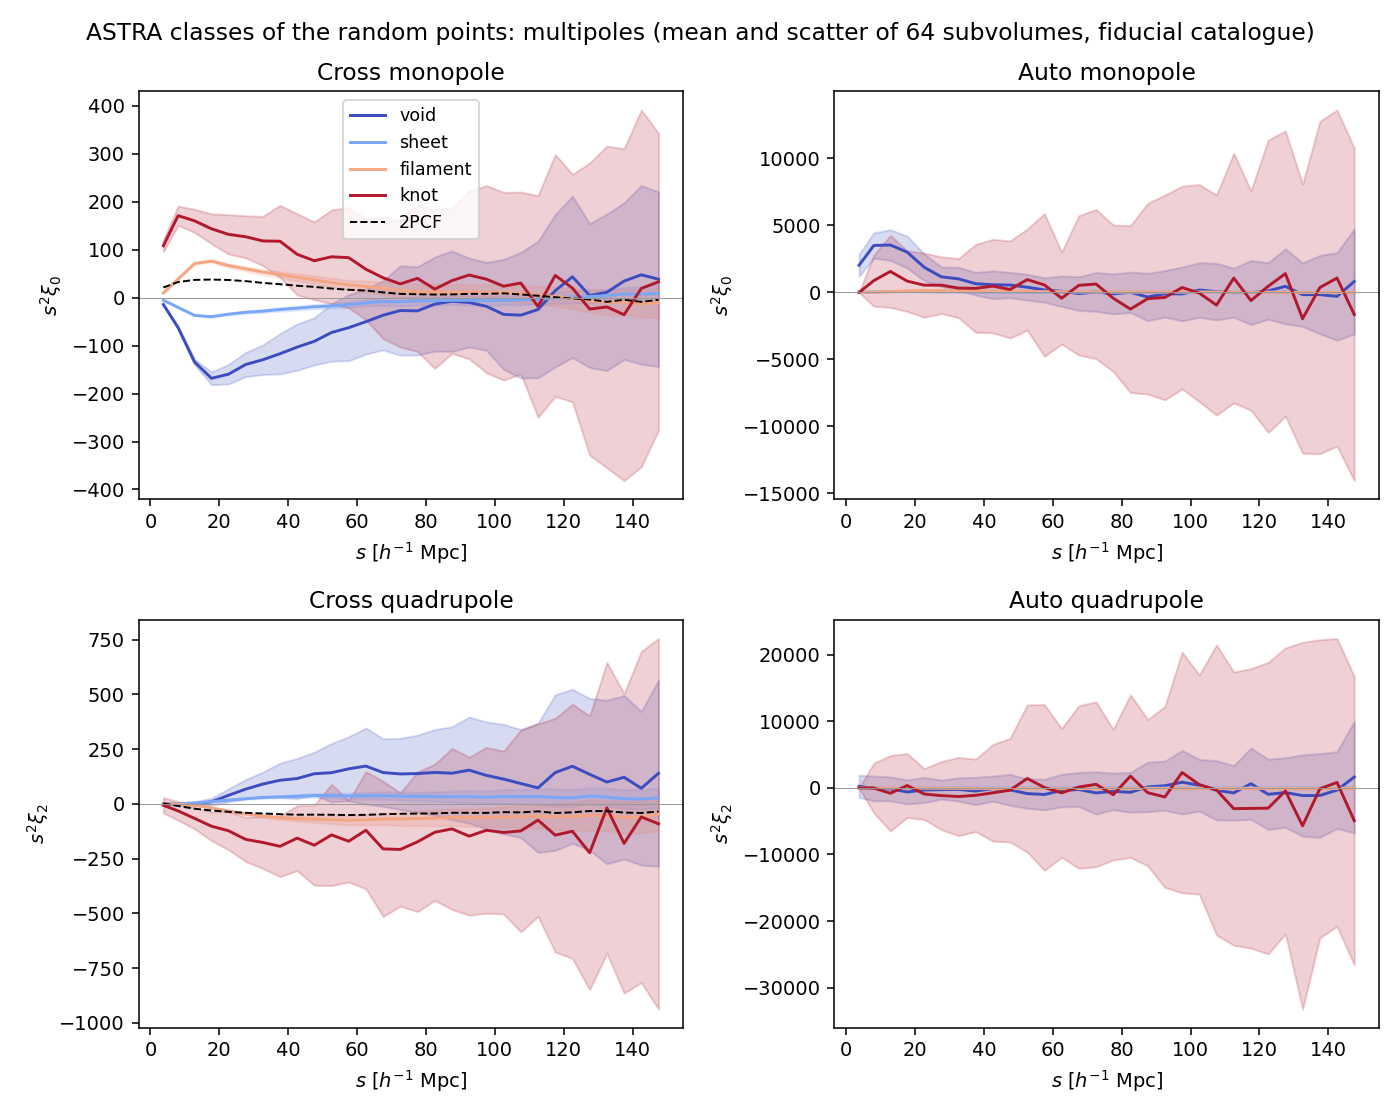
\includegraphics[width=\textwidth]{classes_abacus_multipoles.png}
\caption{Monopole (top) and quadrupole (bottom) of the ASTRA classes of the random points on the fiducial catalogue: cross-correlation with the galaxies (left) and auto-correlation (centre) of the sheets and filaments, and cross-correlation of the voids and knots (right, different scale). Lines and bands: mean and $1\sigma$ scatter of the 64 subvolumes; dashed: 2PCF. The filaments behave like the overdense quartile Q4 and the sheets like the underdense quartile Q1; the voids and knots contain only $\sim150$ and $\sim30$ random points per subvolume, hence their large scatter.}
\label{fig:classes_mp}
\end{figure*}

\subsection{Comparison of the two classifications}

Figure~\ref{fig:env} compares the two estimators on the fiducial catalogue. They are strongly but not perfectly correlated: the Spearman rank correlation between $r$ and $\delta_R$ is $0.719\pm0.005$ for random points and $0.713\pm0.005$ for galaxies (scatter over subvolumes). The extreme quartiles are the most consistent: 63\% of the ASTRA Q1 (Q4) random points are also in the density-split Q1 (Q4), whereas the intermediate quartiles are largely mixed, and less than 2\% of the points move between the two extremes. ASTRA identifies the same large-scale structures as density split but redistributes many points (Figure~\ref{fig:map}), as expected from an adaptive rather than a fixed scale. The distributions of $r$ and $\delta_R$ per quartile are shown in Figure~\ref{fig:envhist}.

\paragraph{Response to cosmology.} Figure~\ref{fig:response} shows how the mean environment of each quartile of the Quijote halos shifts when a cosmological parameter is varied, in units of its scatter between realisations. The density-split contrast $\delta_R$ responds strongly (up to $7\sigma$ for $\sigma_8$), antisymmetrically for the $\pm$ variations; the ASTRA value $r$ hardly moves ($<1\sigma$). This is expected: $r$ is normalised locally by the random points and is nearly insensitive to the overall amplitude of the field. The cosmological information of ASTRA split therefore lies in the clustering of its environments rather than in the values of $r$.

\begin{figure*}[!tp]
\centering
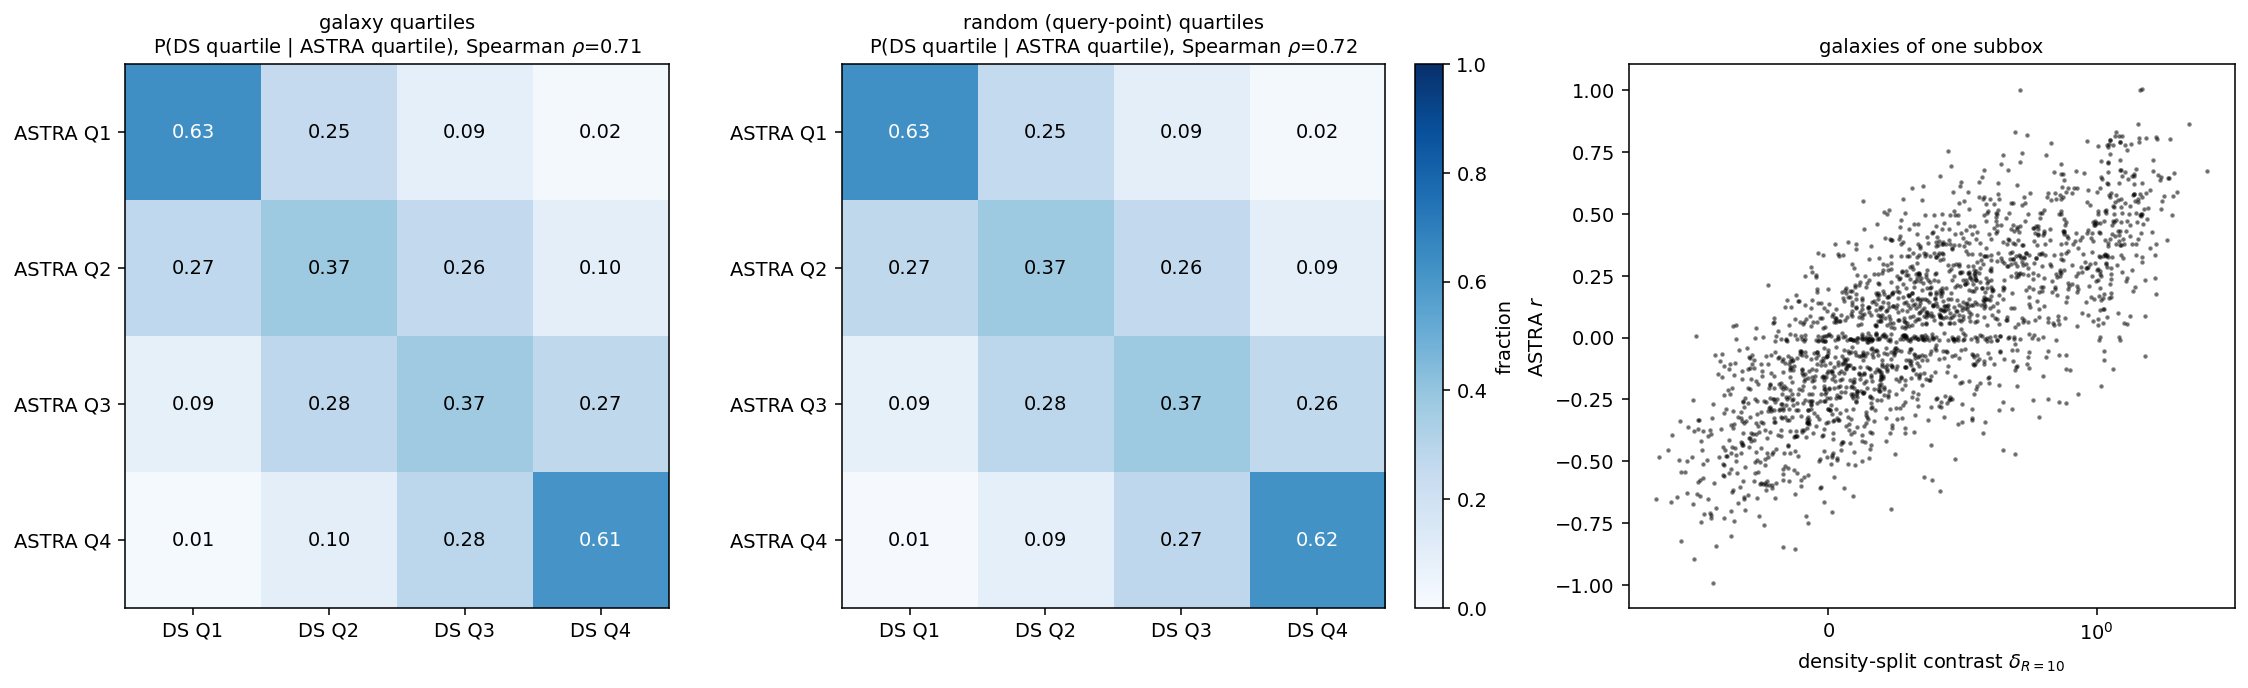
\includegraphics[width=0.95\textwidth]{v2_environment.png}
\caption{ASTRA and density-split environments on the fiducial catalogue (\texttt{c000}, \texttt{hod239}, line of sight $z$). Left, middle: probability that a point of a given ASTRA quartile falls in each density-split quartile, for galaxies and random points (average over 64 subvolumes). Right: ASTRA $r$ against the smoothed density contrast for a sample of galaxies (small vertical jitter added to the discrete $r$).}
\label{fig:env}
\end{figure*}

\begin{figure*}[!tp]
\centering
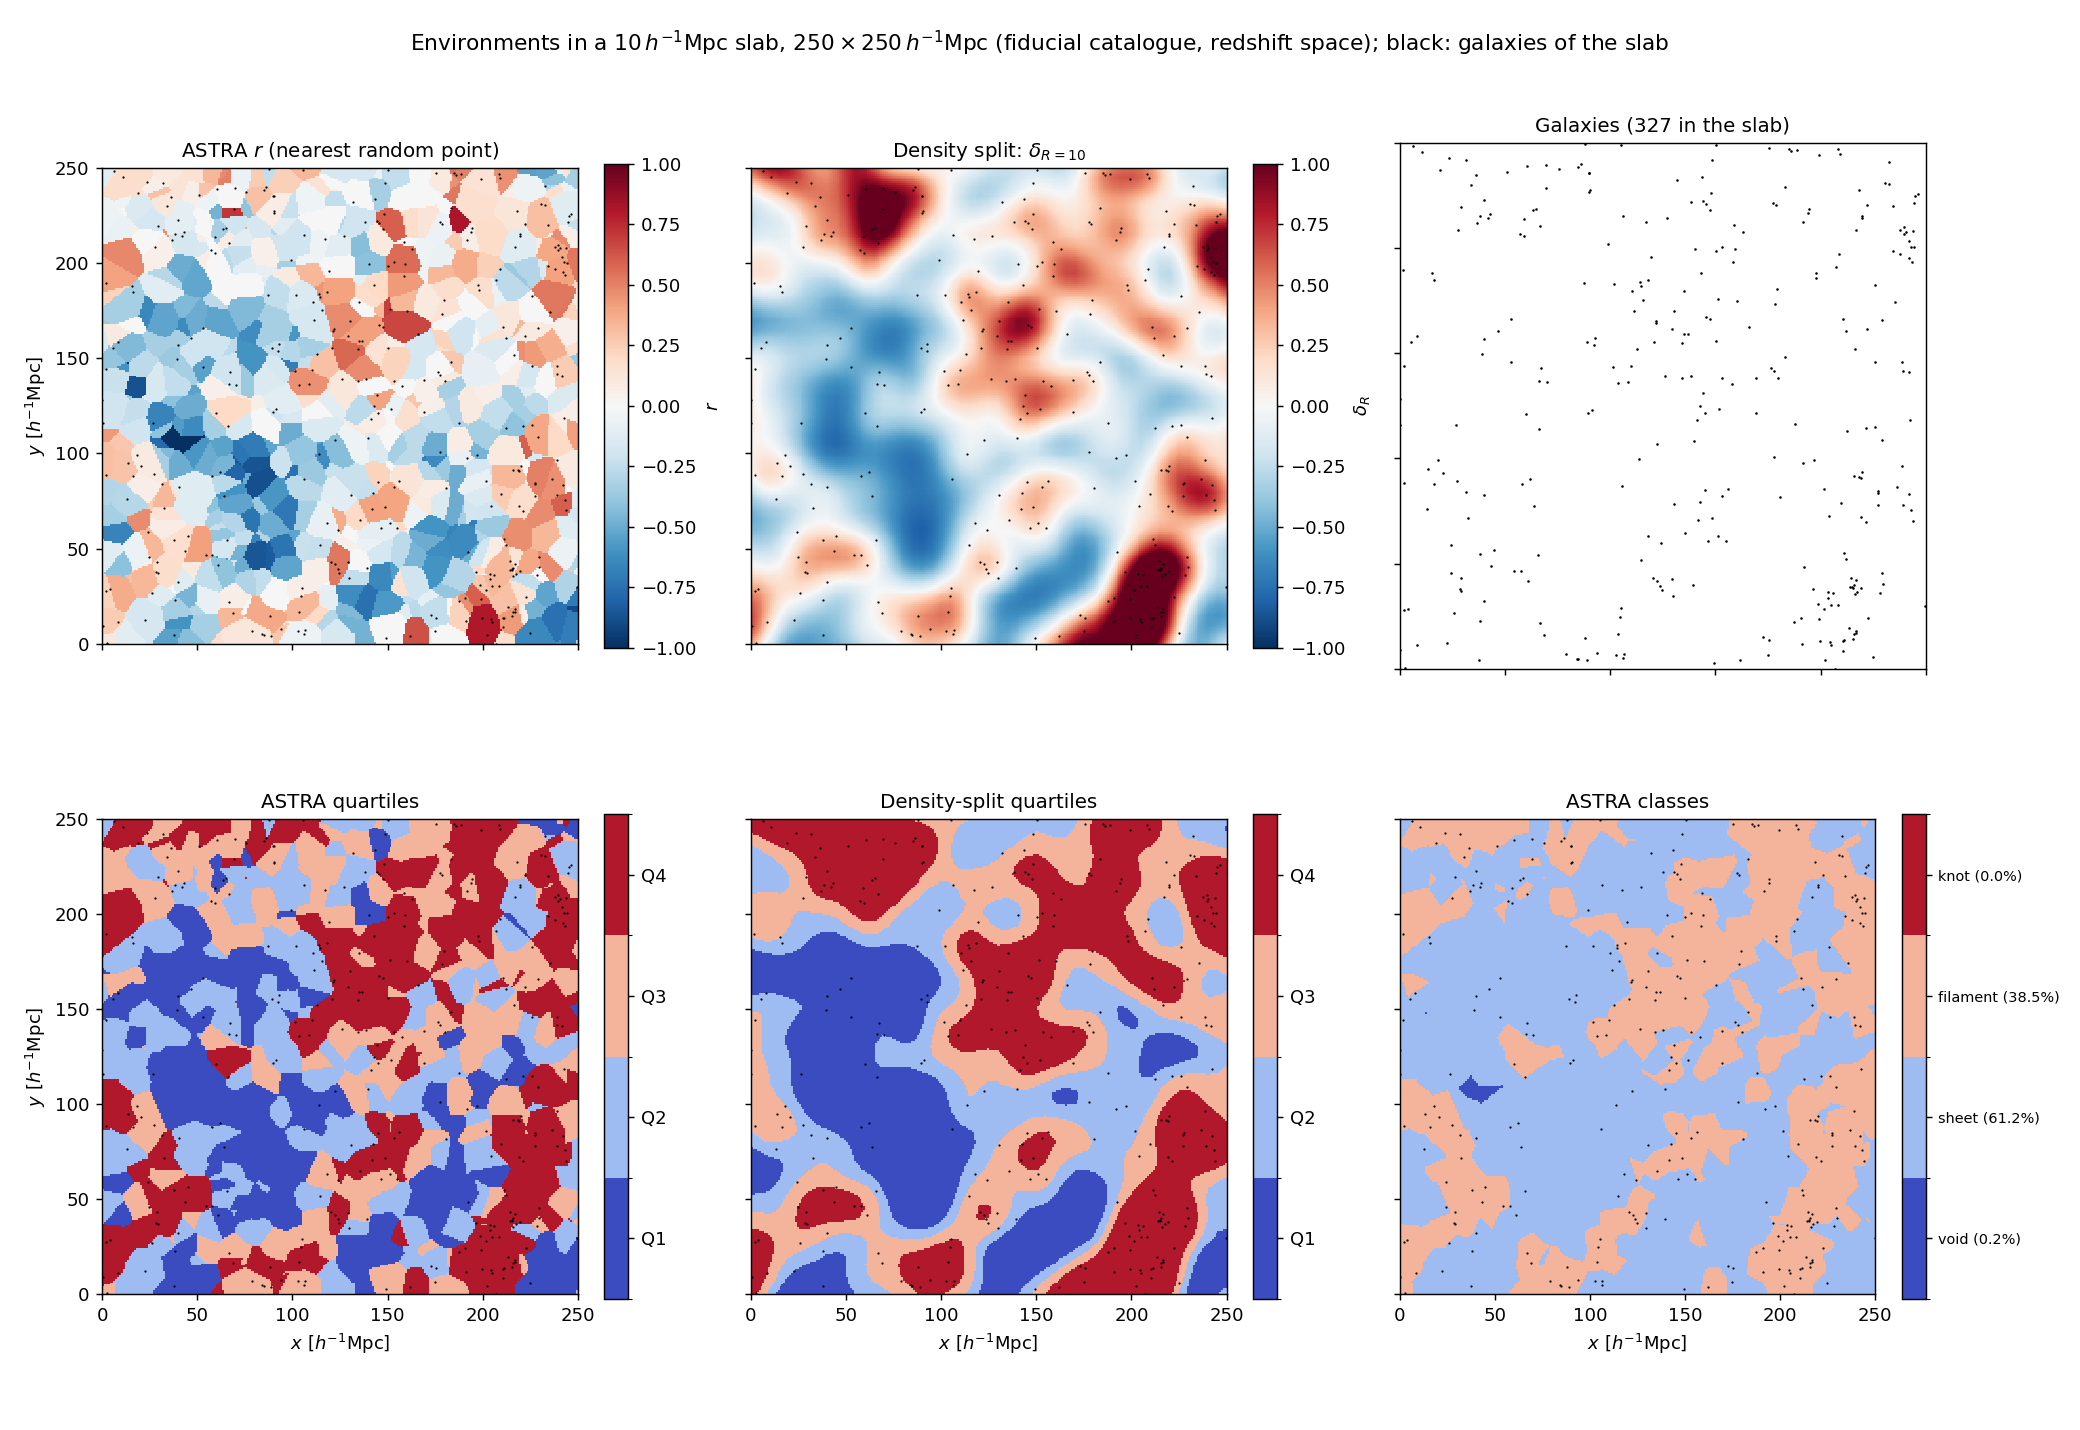
\includegraphics[width=\textwidth]{env_maps.png}
\caption{Environments in a $10\Mpch$ slab of $250\times250\Mpch$ of the fiducial catalogue, drawn as filled regions: each pixel takes the ASTRA value $r$, quartile or class of the nearest random point (left, bottom right), or the smoothed density contrast and its quartile (centre); black dots: galaxies of the slab. ASTRA defines environments cell by cell, at the scale of the Delaunay neighbours, whereas density split defines them on a smooth field; the ASTRA classes are dominated by sheets and filaments.}
\label{fig:map}
\end{figure*}

\begin{figure*}[!tp]
\centering
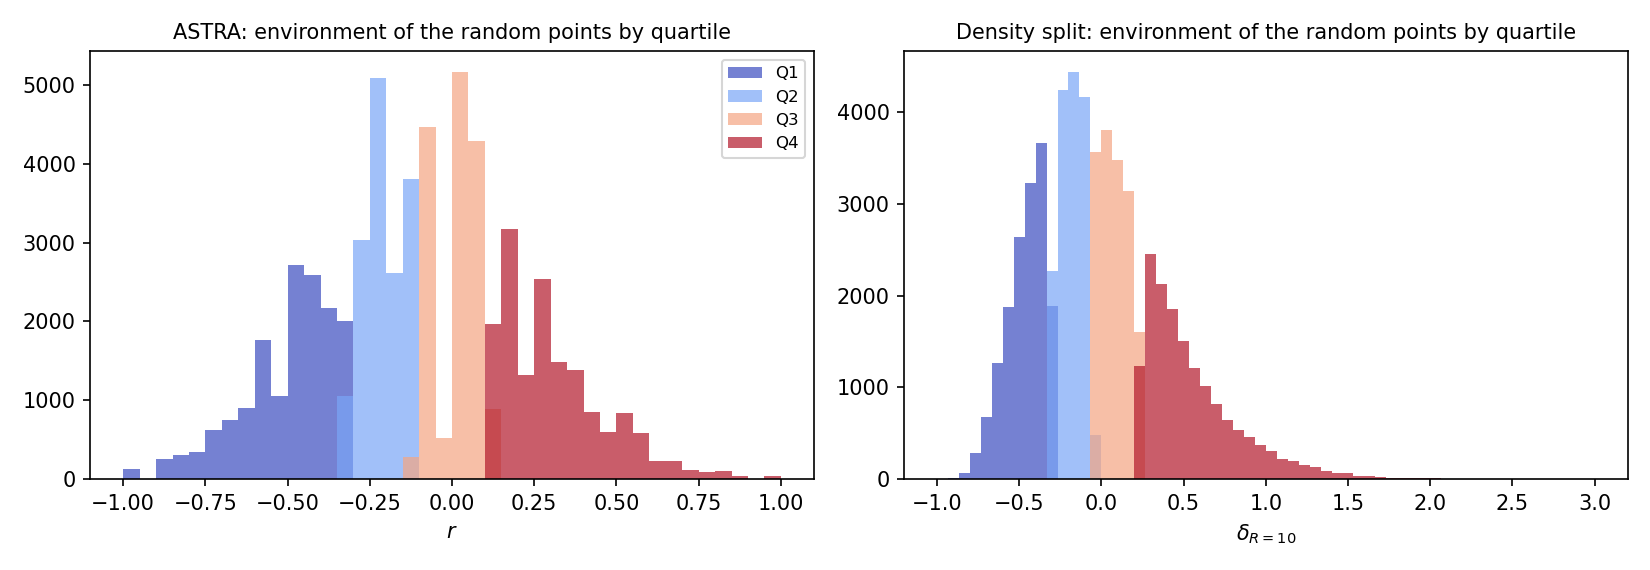
\includegraphics[width=0.85\textwidth]{v2_env_hist.png}
\caption{Distribution of the environment of the random points per quartile: ASTRA $r$ (left, discrete values) and density-split $\delta_R$ (right).}
\label{fig:envhist}
\end{figure*}

\begin{figure*}[!tp]
\centering
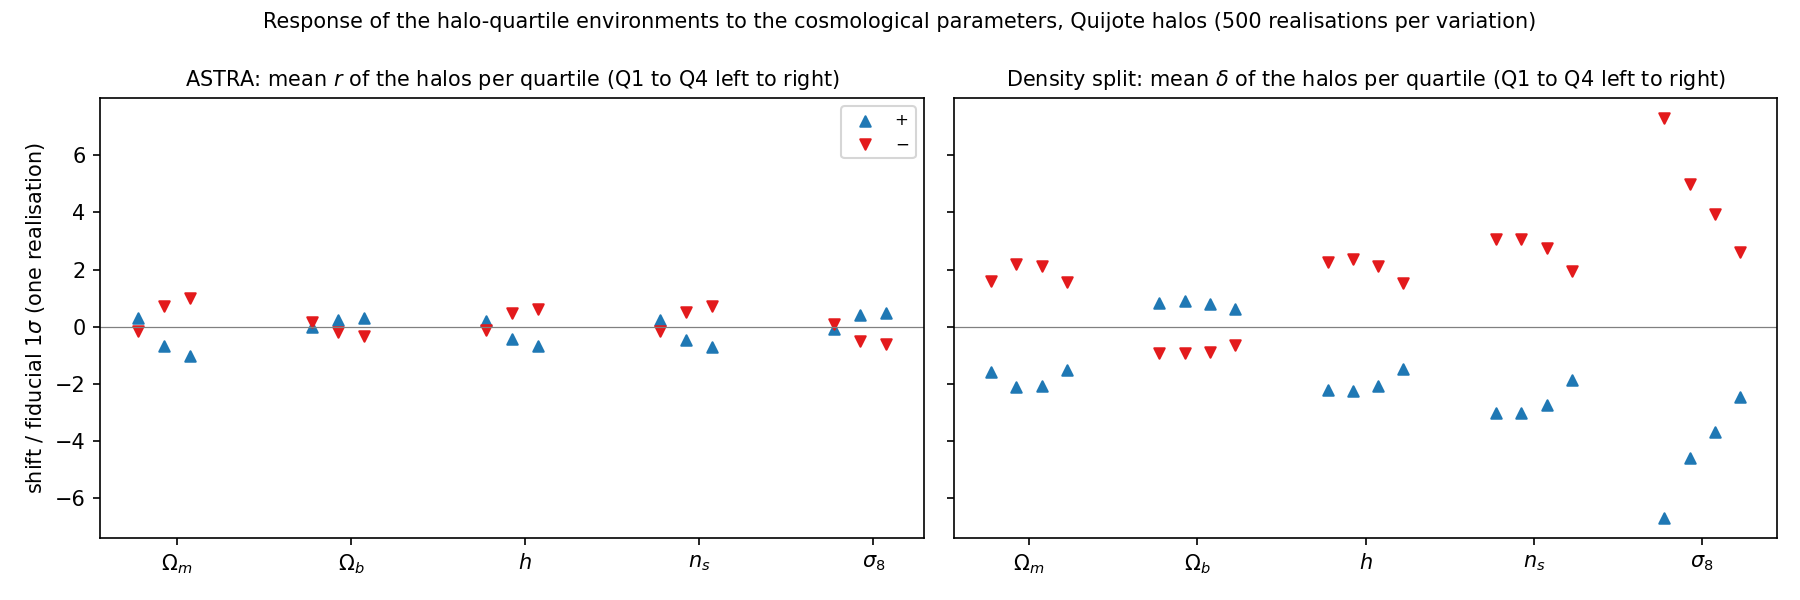
\includegraphics[width=\textwidth]{v2_response.png}
\caption{Shift of the mean environment of each halo quartile (Q1 to Q4 from left to right) for the $+$ (blue) and $-$ (red) variations of each parameter, Quijote, in units of the scatter of one realisation. Left: ASTRA $r$; right: density-split $\delta_R$.}
\label{fig:response}
\end{figure*}


